\documentclass[tikz]{standalone}
\usepackage{palatino,amsbsy}
\usetikzlibrary{calc}
\usetikzlibrary{shapes}
\usetikzlibrary{calc,decorations.pathmorphing,patterns}

\makeatletter

\pgfdeclaredecoration{penciline}{initial}{
    \state{initial}[width=+\pgfdecoratedinputsegmentremainingdistance,auto corner on length=1mm,]{
        \pgfpathcurveto%
        {% From
            \pgfqpoint{\pgfdecoratedinputsegmentremainingdistance}
                            {\pgfdecorationsegmentamplitude}
        }
        {%  Control 1
        \pgfmathrand
        \pgfpointadd{\pgfqpoint{\pgfdecoratedinputsegmentremainingdistance}{0pt}}
                        {\pgfqpoint{-\pgfdecorationsegmentaspect\pgfdecoratedinputsegmentremainingdistance}%
                                        {\pgfmathresult\pgfdecorationsegmentamplitude}
                        }
        }
        {%TO 
        \pgfpointadd{\pgfpointdecoratedinputsegmentlast}{\pgfpoint{1pt}{1pt}}
        }
    }
    \state{final}{}
}
\makeatother

\usepackage{tkz-euclide}
\usetikzlibrary{through}  
\newcommand{\tikzAngleOfLine}{\tikz@AngleOfLine}
\def\tikz@AngleOfLine(#1)(#2)#3{%
\pgfmathanglebetweenpoints{%
\pgfpointanchor{#1}{center}}{%
\pgfpointanchor{#2}{center}}
\pgfmathsetmacro{#3}{\pgfmathresult}%
} 

\def\roundloop[#1]#2#3{%
 \coordinate (rla) at (#2.east); 
 \path   (#2)--++(#1) coordinate (rlb);
 \tkzTgtFromP(#2,rla)(rlb)            
 \node (rlb) at (rlb) [circle through={(tkzFirstPointResult)}] {};
 \coordinate  (rlc) at (intersection 2 of #2 and rlb);
 \coordinate  (rld) at (intersection 1 of #2 and rlb);         
 \tikzAngleOfLine(rlb)(rld){\AngleStart}
 \tikzAngleOfLine(rlb)(rlc){\AngleEnd} 
 \tikzAngleOfLine(#2)(rlb){\AngleLabel}
 \ifdim\AngleStart pt<\AngleEnd pt
 \draw[red,thick,->]%
   let \p1 = ($ (rlb) - (rld) $), \n2 = {veclen(\x1,\y1)}
   in   
     (rlb) ++(\AngleLabel:\n2) node[fill=white]{#3}
     (rld) arc (\AngleStart:\AngleEnd:\n2); 
 \else 
  \draw[red,thick,->]%
   let \p1 = ($ (rlb) - (rld) $), \n2 = {veclen(\x1,\y1)}
   in   
     (rlb) ++(\AngleLabel:\n2) node[fill=white]{#3}
     (rld) arc (\AngleStart-360:\AngleEnd:\n2); 
   \fi 
  }

\begin{document}
 \pgfkeys{/pgf/decoration/.cd,
      distance/.initial=10pt
}  

\pgfdeclaredecoration{add dim}{final}{
\state{final}{% 
\pgfmathsetmacro{\dist}{5pt*\pgfkeysvalueof{/pgf/decoration/distance}/abs(\pgfkeysvalueof{/pgf/decoration/distance})} 
          \pgfpathmoveto{\pgfpoint{0pt}{0pt}}             
          \pgfpathlineto{\pgfpoint{0pt}{2*\dist}}   
          \pgfpathmoveto{\pgfpoint{\pgfdecoratedpathlength}{0pt}} 
          \pgfpathlineto{\pgfpoint{(\pgfdecoratedpathlength}{2*\dist}}
           \pgfusepath{stroke} 
          \pgfsetdash{{0.1cm}{0.1cm}{0.1cm}{0.1cm}}{0cm}     
          \pgfsetarrowsstart{latex}
          \pgfsetarrowsend{latex}  
          \pgfpathmoveto{\pgfpoint{0pt}{\dist}}
          \pgfpathlineto{\pgfpoint{\pgfdecoratedpathlength}{\dist}} 
          \pgfusepath{stroke} 
          \pgfsetdash{}{0pt}
          \pgfpathmoveto{\pgfpoint{0pt}{0pt}}
          \pgfpathlineto{\pgfpoint{\pgfdecoratedpathlength}{0pt}}
}}

\tikzset{dim/.style args={#1,#2}{decoration={add dim,distance=#2},
                decorate,
                postaction={decorate,decoration={text along path,
                                                 raise=#2,
                                                 text align={align=center},
                                                 text={#1}}}}}

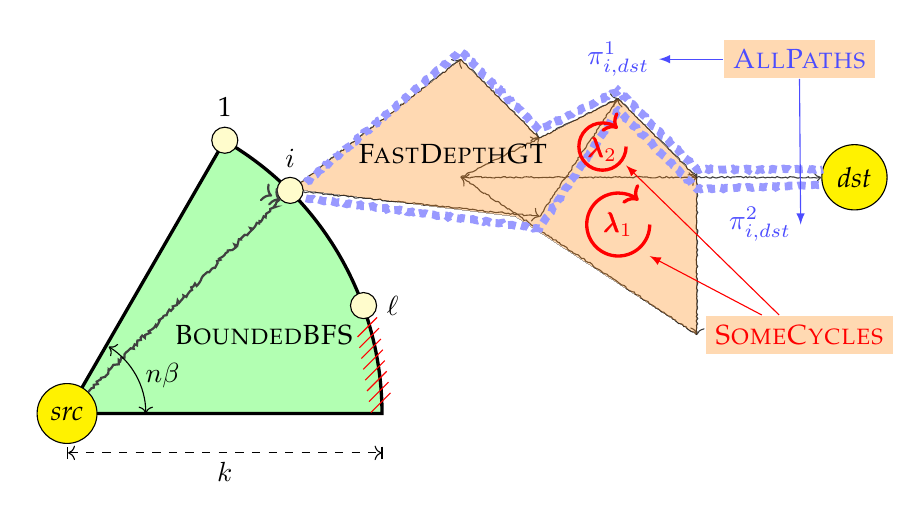
\begin{tikzpicture}[pencildraw/.style={
    black!75,
    decorate,
    decoration={random steps,segment length=0.8pt,amplitude=0.3pt}},
fpencildraw/.style={
    black!75,
    decorate,
    decoration={random steps,segment length=0.8pt,amplitude=0.7pt}}]


  \clip (-.5,-1) rectangle (10.5,4.9);
\draw[very thick,fill=green!30] (0,0) --  (0:4) arc(0:60:4) -- cycle;
\node[circle,draw,fill=yellow] (src) {\textit{src}};

\node [circle, minimum size=8cm] (c) {};
      \node[circle, draw, minimum width=1,fill=yellow!20,
            label=1] (one) at (c.60) {};

\node [circle, minimum size=8cm] (c) {};
      \node[circle, draw, minimum width=1,fill=yellow!20,
            label=$i$] (two) at (c.45) {};

      \node[circle, draw, minimum width=1,fill=yellow!20,
            label=right:$\ell$] at (c.20) {};

\draw[fpencildraw,draw,->>,thick] (src) -- (two);

\draw [<->]  (0:1)   arc (0:58:1)   node[midway, right]{$n\beta$};

\node at (2.5,1) {\textsc{BoundedBFS}};
\node[fill=orange!30] (ac) at (9.3,1) {\textsc{\color{red}SomeCycles}};

\draw[draw=black,dashed,|<->|] ($(c)-(0,0.5)$) -- ($(c.0)-(0,0.5)$) node [midway,below] {$k$};


  \path (c.0) -- (c.20) node[draw,strike out, pos=0.1,draw=red] {}
                        node[draw,strike out, pos=0.2,draw=red] {}
                        node[draw,strike out, pos=0.3,draw=red] {}
                        node[draw,strike out, pos=0.4,draw=red] {}
                        node[draw,strike out, pos=0.5,draw=red] {}
                        node[draw,strike out, pos=0.6,draw=red] {}
                        node[draw,strike out, pos=0.7,draw=red] {}
                        node[draw,strike out, pos=0.8,draw=red] {};

\node[circle,draw,fill=yellow]  at (10,3) (dst) {\textit{dst}};

\coordinate (a) at (5,4.5);
\coordinate (b) at (6,3.5);
\coordinate (d) at (7,4);
\coordinate (e) at (8,3);
\coordinate (f) at (6,2.5);
\coordinate (g) at (8,1);
\coordinate (h) at (5,3);

\draw[pencildraw,draw,->] (two)--(a);
\draw[pencildraw,draw,->] (a)--(b);
\draw (b) edge[pencildraw,draw,->] (d);
\draw (d) edge[pencildraw,draw,->] (e);
\draw (e) edge[pencildraw,draw,->] (dst);
\draw  (two) edge[draw,pencildraw,->] (f);
\draw  (f) edge[draw,pencildraw,->] (d);
\draw  (e) edge[draw,pencildraw,->] (g);
\draw  (g) edge[draw,pencildraw,->] (h);
\draw  (h) edge[draw,pencildraw,->] (b);
\draw  (h) edge[draw,pencildraw,->] (e);
\draw[fill=orange,opacity=.3,line width=0mm] (two) -- (a) -- (b) -- (d) -- (e) -- (g) -- (5.7,2.5) -- (two.east) -- cycle; 

\draw[line width=.1cm,pencildraw,draw,dotted,color=blue!40] ($(two)+(.2,.1)$) -- ($(a)+(0,.1)$) -- ($(b)+(0,.1)$) -- ($(d)+(0,.1)$) -- ($(e)+(0,.1)$) -- ($(dst)+(-.4,.1)$);
\draw[line width=.1cm,pencildraw,draw,dotted,color=blue!40] ($(two)-(-.2,.1)$) -- ($(f)-(0,.15)$) -- ($(d)-(0,.15)$) -- ($(e)-(0,.15)$) -- ($(dst)-(.4,.1)$);

\node (p1) at (7,4.5) {$\color{blue!70}\pi_{i,{dst}}^1$};
\node[fill=orange!30] (ap) at (9.3,4.5) {\textsc{\color{blue!70}AllPaths}};
\node (p2) at (8.8,2.4) {$\color{blue!70}\pi_{i,{dst}}^2$};
 
	\node (l1) at (7,2.4) {$\color{red}\pmb{\lambda}_1$};
	\node (l2) at (6.8,3.35) {$\color{red}\pmb{\lambda}_2$};
    \draw [->,very thick, red] (7.4,2.4) arc (0:-310:.4 cm);
    \draw [->,very thick, red] (7.1,3.39) arc (0:-310:.3 cm);

\node at (4.9,3.3) {\textsc{FastDepthGT}};
\draw[red,latex-] ($(l1)+(.4,-.4)$)--(ac);
\draw[red,latex-] ($(l2)+(.3,-.2)$)--(ac);
\draw[blue!70,latex-] (p1)--(ap);
\draw[blue!70,latex-] (p2.east)--(ap);
\end{tikzpicture}
\end{document}